\section{Simulación}

El modelo matemático obtenido se implementó en MATLAB 
para estudiar el comportamiento del sistema.
La tabla \ref{table: simulation conditions}
muestra las condiciones de simulación del programa.
Los resultados de la simulación pueden ser 
observados en las figuras \ref{fig: time plot theta dtheta}
 y \ref{fig: phase plot theta}. 
El código del programa se encuentra disponible en 
Github\footnote{\url{https://github.com/der-coder/Cinvestav-SystemModeling-project/tree/master/codigosM}}
y se incluye como anexo.

\begin{table}[hb]
 \begin{center}
\begin{tabular}{lc}
\hline
Longitud ($l$) & 2.5 [m] \\
Masa ($m$) & 5 [kg]\\
Coeficiente de fricción ($k$) & 1 [$N \cdot s / m$] \\
Posición angular inicial ($\theta_0$) & $0.5\pi$ [rad] \\
Velocidad angular inicial ($\dot{\theta}$) & 0 [rad/s] \\
Tiempo de simulación & 15 [s]  \\
Gravedad ($g$) & 9.81 [$m/s^2$]  \\
\hline
 \end{tabular}
 \end{center}
 \caption{Condiciones de simulación del sistema.}
\label{table: simulation conditions}
\end{table}


Se observa que el péndulo tiende a una posición de reposo debido
al efecto que la fuerza de fricción tiene sobre el sistema.
El péndulo comienza en la posición angular máxima posible 
($\theta_{max}$) y la amplitud de las crestas y valles de las 
ecuaciones disminuye para cada período de oscilación.
El diagrama de fase confirma esta tendencia, la curva del sistema
indica que tiende a un punto de estabilización en $\theta = 0$,
posicionando al péndulo en el eje vertical del marco referencial.

\begin{figure}[hb]
 \centering 
 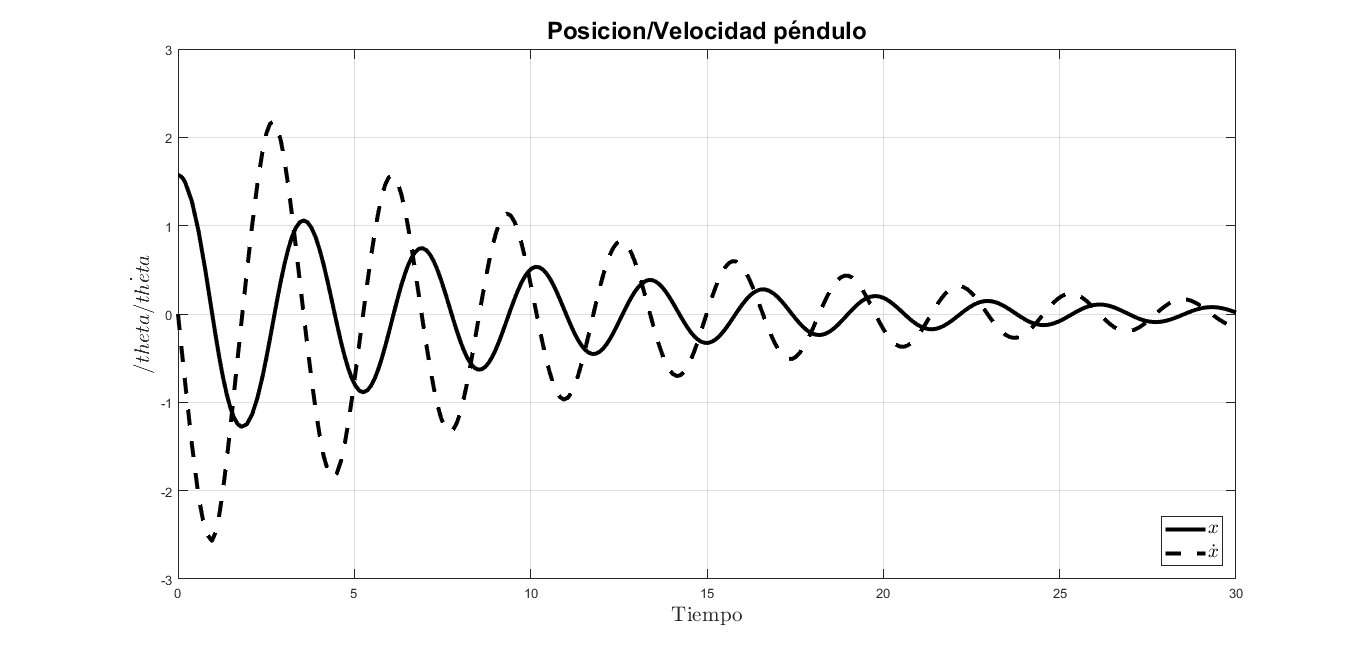
\includegraphics[scale=0.35]{./img/posvelpendulo2.png}
 % fasependulox2.png: 1853x1003 px, 96dpi, 49.02x26.53 cm, bb=0 0 1390 752
 \caption{Comportamiento de $\theta(t)$ y $\dot{\theta}(t)$ en el tiempo.}
 \label{fig: time plot theta dtheta}
\end{figure}

\begin{figure}[hb]
 \centering 
 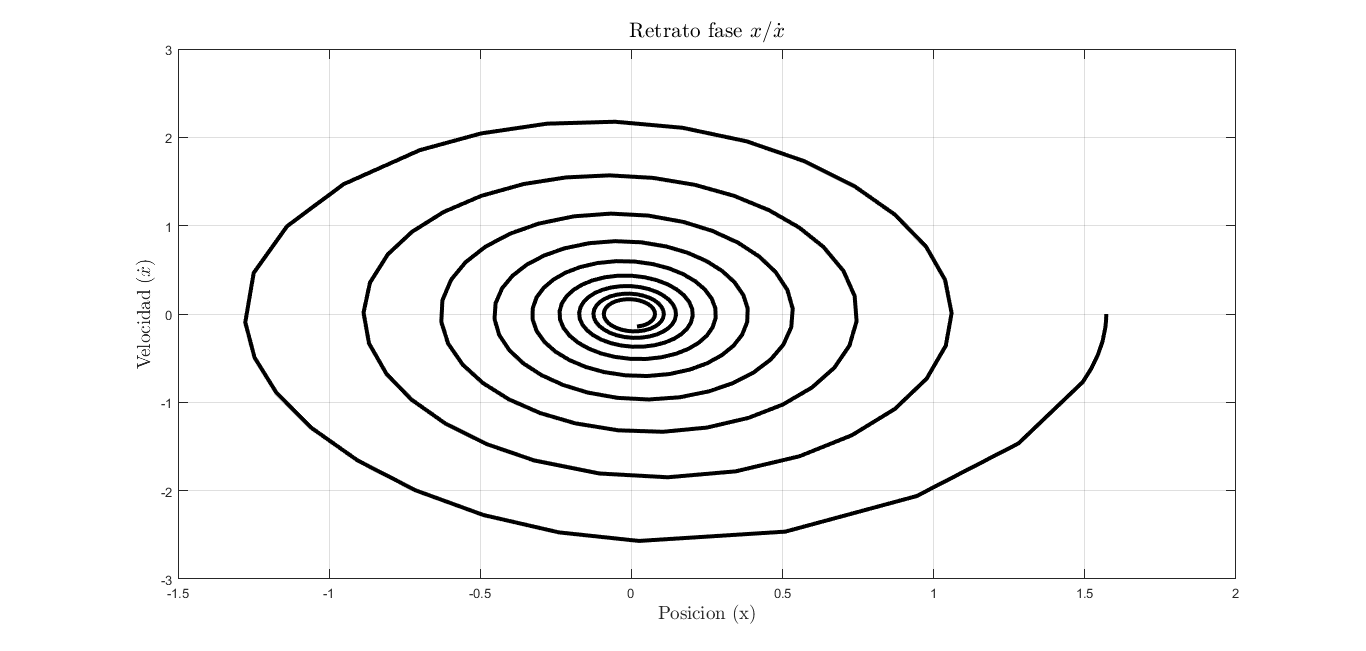
\includegraphics[scale=0.35]{./img/fasependulox2.png}
 % fasependulox2.png: 1853x1003 px, 96dpi, 49.02x26.53 cm, bb=0 0 1390 752
\caption{Diagrama de fase de $\theta(t)$ y $\dot{\theta}(t)$.}
 \label{fig: phase plot theta}
\end{figure}



